\documentclass[aspectratio=169]{beamer}

\usepackage[utf8]{inputenc}
\usepackage[T1]{fontenc}
\usepackage[croatian]{babel}
\usepackage{graphicx}
\usepackage{amsmath}

\usetheme{Madrid}
\usecolortheme{seahorse}
\graphicspath{{figures/}}

\title[Kratki spojevi --- simetrične mreže]{Proračun kratkih spojeva za transmisione mreže\\(simetrične mreže)}
\author[I. Erović]{Ilhan Erović}
\institute[ETF Sarajevo]{Univerzitet u Sarajevu --- Elektrotehnički fakultet\\Seminarski rad iz predmeta SREES}
\date{2026}

\begin{document}

\begin{frame}[plain]
  \titlepage
\end{frame}

\begin{frame}{Uvod}
  \begin{itemize}
    \item Kratki spoj $\Rightarrow$ nagli \textbf{porast struje} i \textbf{pad napona}.
    \item Može oštetiti opremu i ugroziti stabilnost sistema.
    \item Proračun kvara je osnova za:
      \begin{itemize}
        \item dimenzionisanje prekidača,
        \item podešavanje relejne zaštite,
        \item provjeru izdržljivosti opreme.
      \end{itemize}
    \item Tema rada: \textbf{simetrični (tropolni)} kvar --- sve tri faze
      simetrično zahvaćene $\Rightarrow$ jednofazni ekvivalent (pozitivni redoslijed).
  \end{itemize}
\end{frame}

\begin{frame}{Cilj rada}
  \begin{block}{Zadatak}
    Razviti program koji za proizvoljnu transmisionu mrežu izračunava veličine
    tropolnog kratkog spoja i prikazuje ih tabelarno i grafički.
  \end{block}
  \begin{itemize}
    \item Ulaz: mreža u \textbf{MATPOWER} \texttt{.m} formatu.
    \item Metoda: \textbf{Z-bus} preko rijetke kompleksne matrice.
    \item Grafički interfejs u frameworku \textbf{natID} (C++).
  \end{itemize}
\end{frame}

\begin{frame}{Teorija --- matrica admitansi $\mathbf{Y}_{\text{bus}}$}
  Mreža se opisuje matricom admitansi $N\times N$. Za granu $f\!-\!t$
  ($y=1/(r+jx)$, otočno punjenje $b/2$, tap $a=\tau e^{j\theta}$):
  \[
  Y_{ff}\!\mathrel{+}=\!\frac{y+j\frac{b}{2}}{a\,a^{*}},\;\;
  Y_{tt}\!\mathrel{+}=\!y+j\tfrac{b}{2},\;\;
  Y_{ft}\!\mathrel{+}=\!-\frac{y}{a^{*}},\;\;
  Y_{tf}\!\mathrel{+}=\!-\frac{y}{a}
  \]
  \begin{itemize}
    \item Otočni elementi sabirnica: $Y_{ii}\mathrel{+}=(G_s+jB_s)/S_b$.
    \item \textbf{Generatori}: reaktansa prema zemlji $y_g=1/(jX'_d)$
      (podrazumijevano $X'_d=0{,}0608$ pu).
  \end{itemize}
\end{frame}

\begin{frame}{Z-bus metoda proračuna kvara}
  Za kvar na sabirnici $k$ rješava se linearni sistem
  \[
    \mathbf{Y}_{\text{bus}}\,\mathbf{z}=\mathbf{e}_k \;\Rightarrow\; Z_{kk}=z_k
  \]
  ($k$-ta kolona matrice $\mathbf{Z}_{\text{bus}}=\mathbf{Y}^{-1}$). Uz ravni
  prednapon $V_0=1{,}0$ pu i impedansu kvara $Z_f$:
  \begin{columns}
    \column{0.5\textwidth}
    \[ I_f=\frac{V_0}{Z_{kk}+Z_f} \]
    \[ V_i=V_0-z_i\,I_f \]
    \column{0.5\textwidth}
    \[ I_{ij}=y\Big(\tfrac{V_i}{a}-V_j\Big) \]
    \[ S_k=S_b\,|I_f|_{\text{pu}} \]
  \end{columns}
  \vspace{4pt}
  Doprinos generatora: $I_g=(E-V_g)/(jX'_d)$, \; $E\approx V_0$.
\end{frame}

\begin{frame}{Algoritam}
  \begin{columns}
    \column{0.42\textwidth}
    \begin{enumerate}\small
      \item parsiranje \texttt{.m} datoteke,
      \item formiranje $\mathbf{Y}_{\text{bus}}$,
      \item LU faktorizacija,
      \item rješavanje $\mathbf{Y}\mathbf{z}=\mathbf{e}_k$,
      \item $I_f$, naponi, struje grana, doprinos generatora,
      \item prikaz i izvoz rezultata.
    \end{enumerate}
    \column{0.55\textwidth}
    \centering
    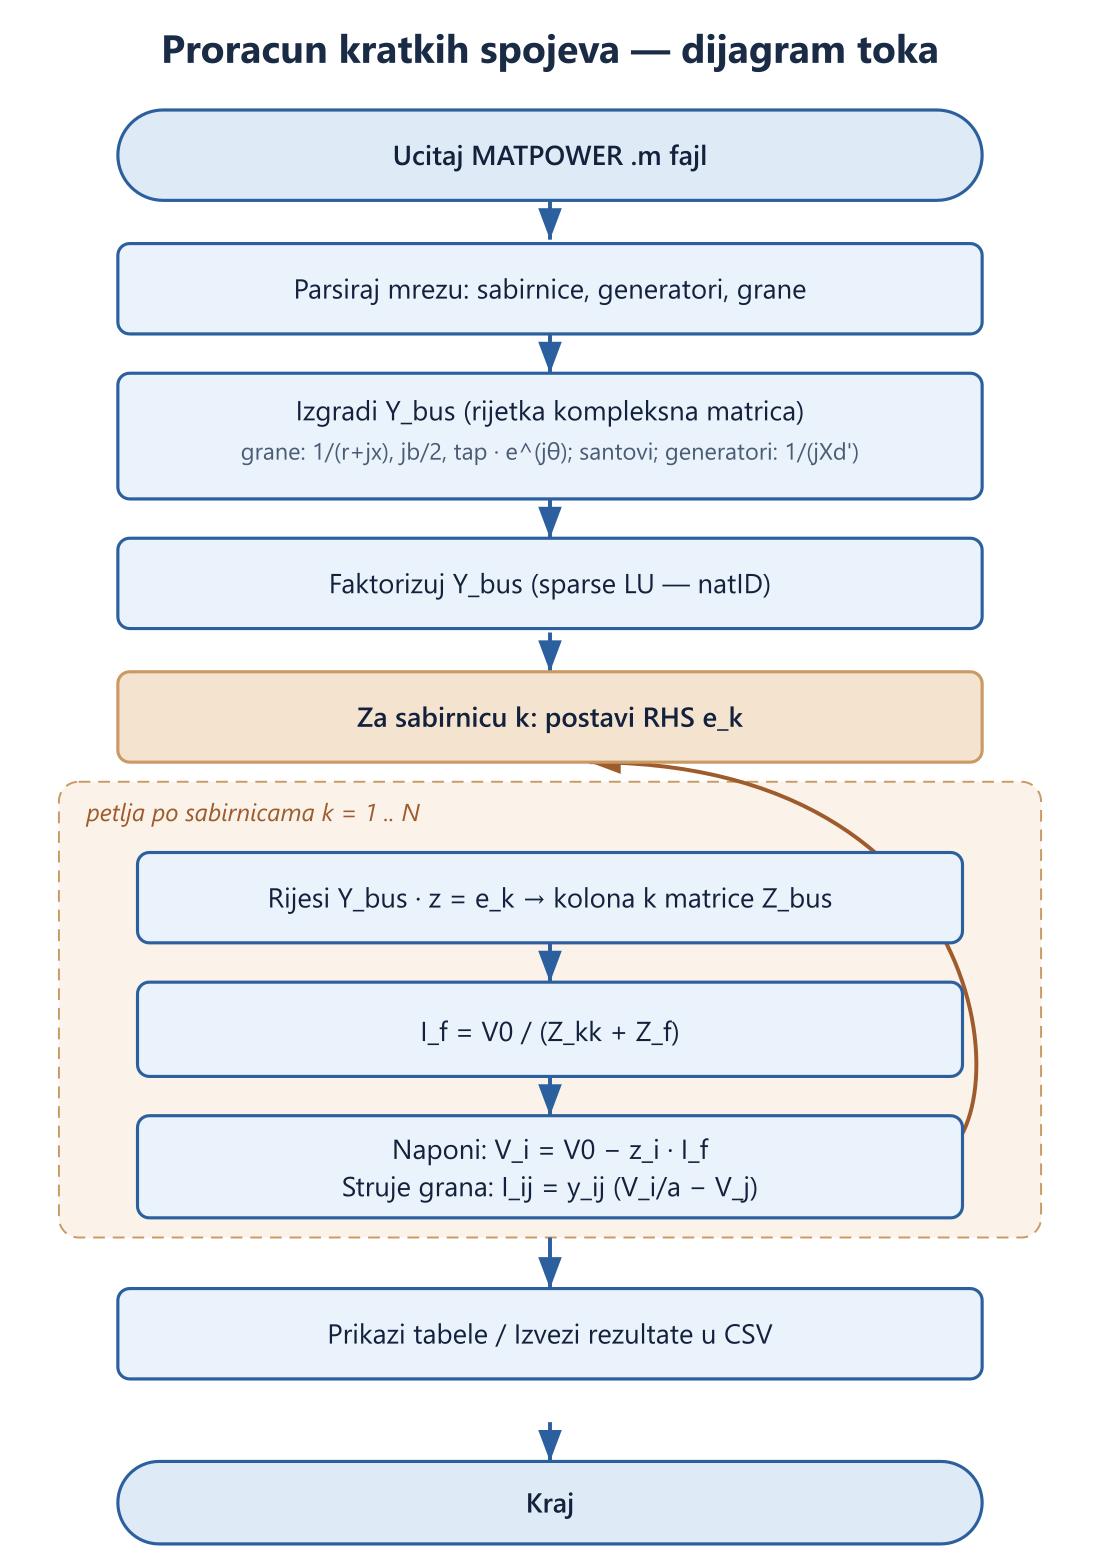
\includegraphics[height=0.75\textheight]{flowchart.png}
  \end{columns}
\end{frame}

\begin{frame}{Implementacija}
  \begin{itemize}
    \item Jezik \textbf{C++}, framework \textbf{natID}; build u \textbf{CMake}
      (Windows/Linux).
    \item Sve matrice = natID klase: $\mathbf{Y}_{\text{bus}}$ \textbf{rijetka
      kompleksna}, vektori \textbf{puni (dense)}.
    \item LU faktorizacija jednom, pa ponovna upotreba za svaku sabirnicu (samo
      mijenja se desna strana).
    \item Struktura:
      \begin{itemize}\small
        \item \texttt{MatpowerParser} --- parsiranje,
        \item \texttt{ShortCircuitSolver} --- $\mathbf{Y}_{\text{bus}}$ + proračun,
        \item GUI --- tabovi, grafici i shema (natID \texttt{Canvas}).
      \end{itemize}
  \end{itemize}
\end{frame}

\begin{frame}{Aplikacija --- grafički interfejs}
  \centering
  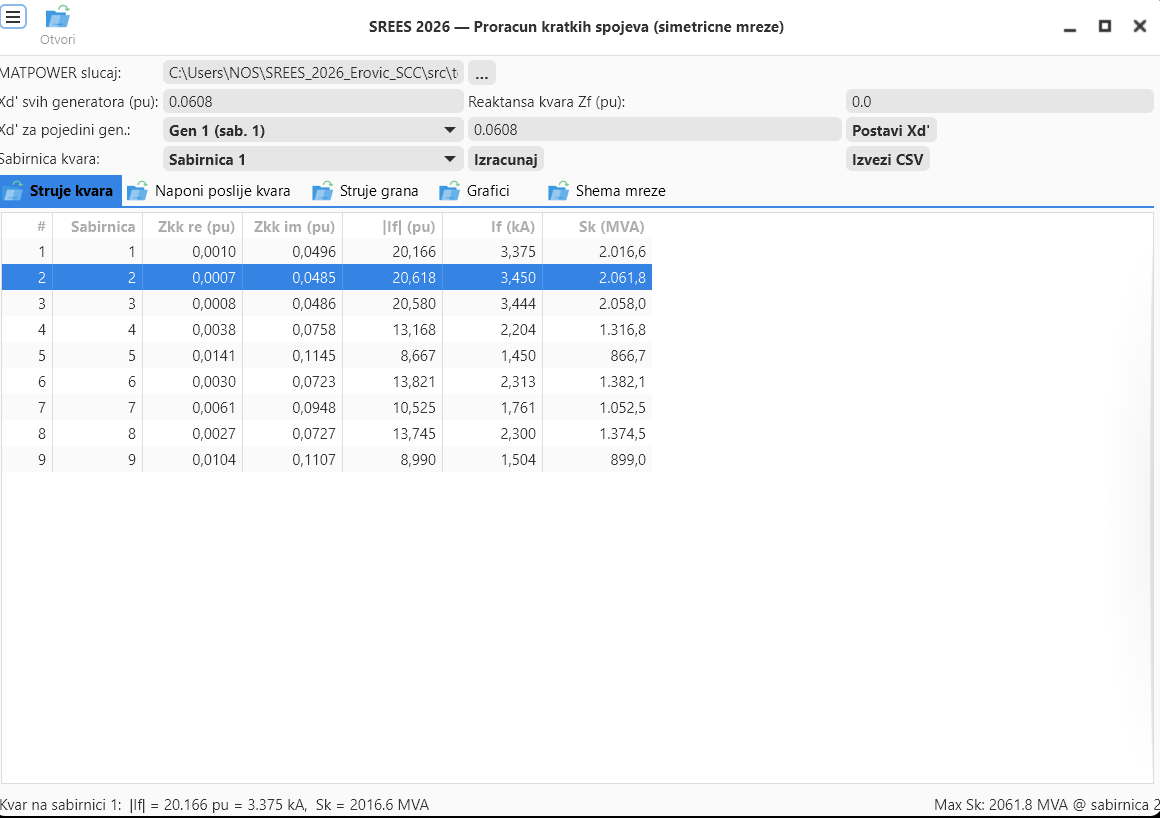
\includegraphics[width=0.95\textwidth]{gui_fault_table.png}
\end{frame}

\begin{frame}{Rezultati --- case9 (kvar na sabirnici 1)}
  \begin{columns}
    \column{0.4\textwidth}
    \begin{itemize}\small
      \item $I_f=20{,}17$ pu $=3{,}38$ kA
      \item $S_k=2016{,}6$ MVA
      \item Doprinos generatora:
        \begin{itemize}
          \item G1: \textbf{79{,}1\,\%}
          \item G2, G3: po 10{,}5\,\%
        \end{itemize}
    \end{itemize}
    \column{0.6\textwidth}
    \centering
    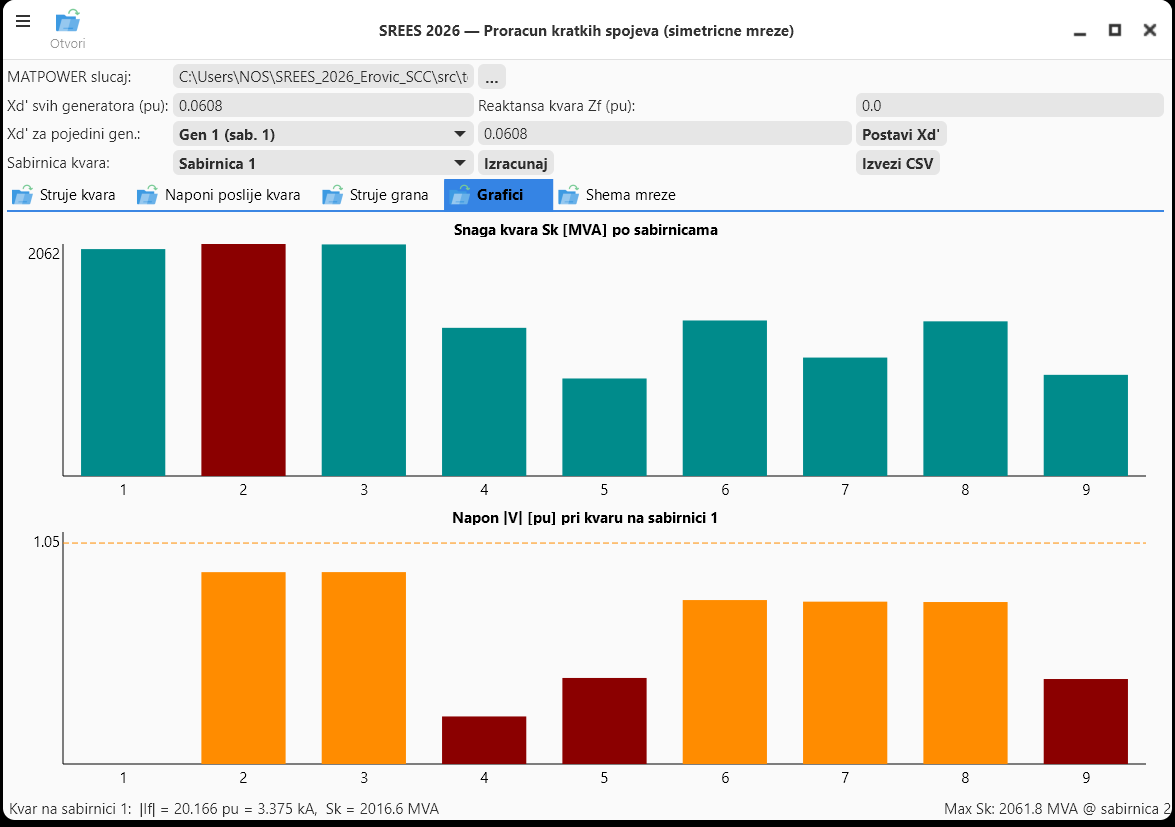
\includegraphics[width=\textwidth]{charts.png}
  \end{columns}
\end{frame}

\begin{frame}{Jednopolna shema s rezultatima}
  \centering
  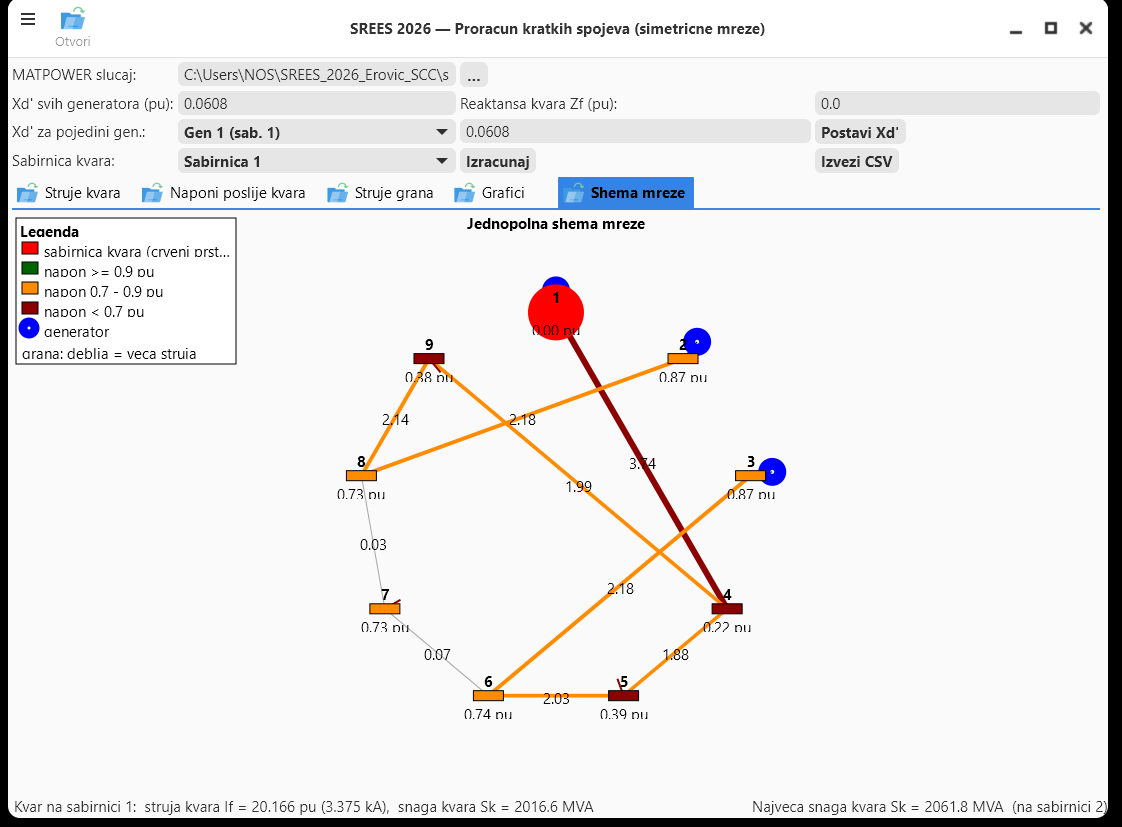
\includegraphics[height=0.82\textheight]{oneline_app.png}
\end{frame}

\begin{frame}{Verifikacija i zaključak}
  \begin{block}{Verifikacija}
    Rezultati ($Z_{kk}$, $I_f$, struje grana) poklapaju se s nezavisnim
    proračunom u MATLAB-u ($\mathbf{Z}=\mathbf{Y}^{-1}$) do na 4 decimale.
  \end{block}
  \begin{itemize}
    \item Razvijen funkcionalan i \textbf{verifikovan} program za simetrični kvar.
    \item Efikasan i na velikim mrežama (do 300 sabirnica).
    \item Numerički rezultati + vizualizacija + izvoz (CSV, PDF/SVG).
  \end{itemize}
  \vspace{6pt}
  \centering \Large Hvala na pažnji!
\end{frame}

\end{document}
